\section{The Lipkin model}

First we show that our implementation of the restricted Boltzmann machine manages to converge towards the ground state energy. With a system size of $25$ particles we get the convergence:

\begin{figure}[H]
  \begin{center}
    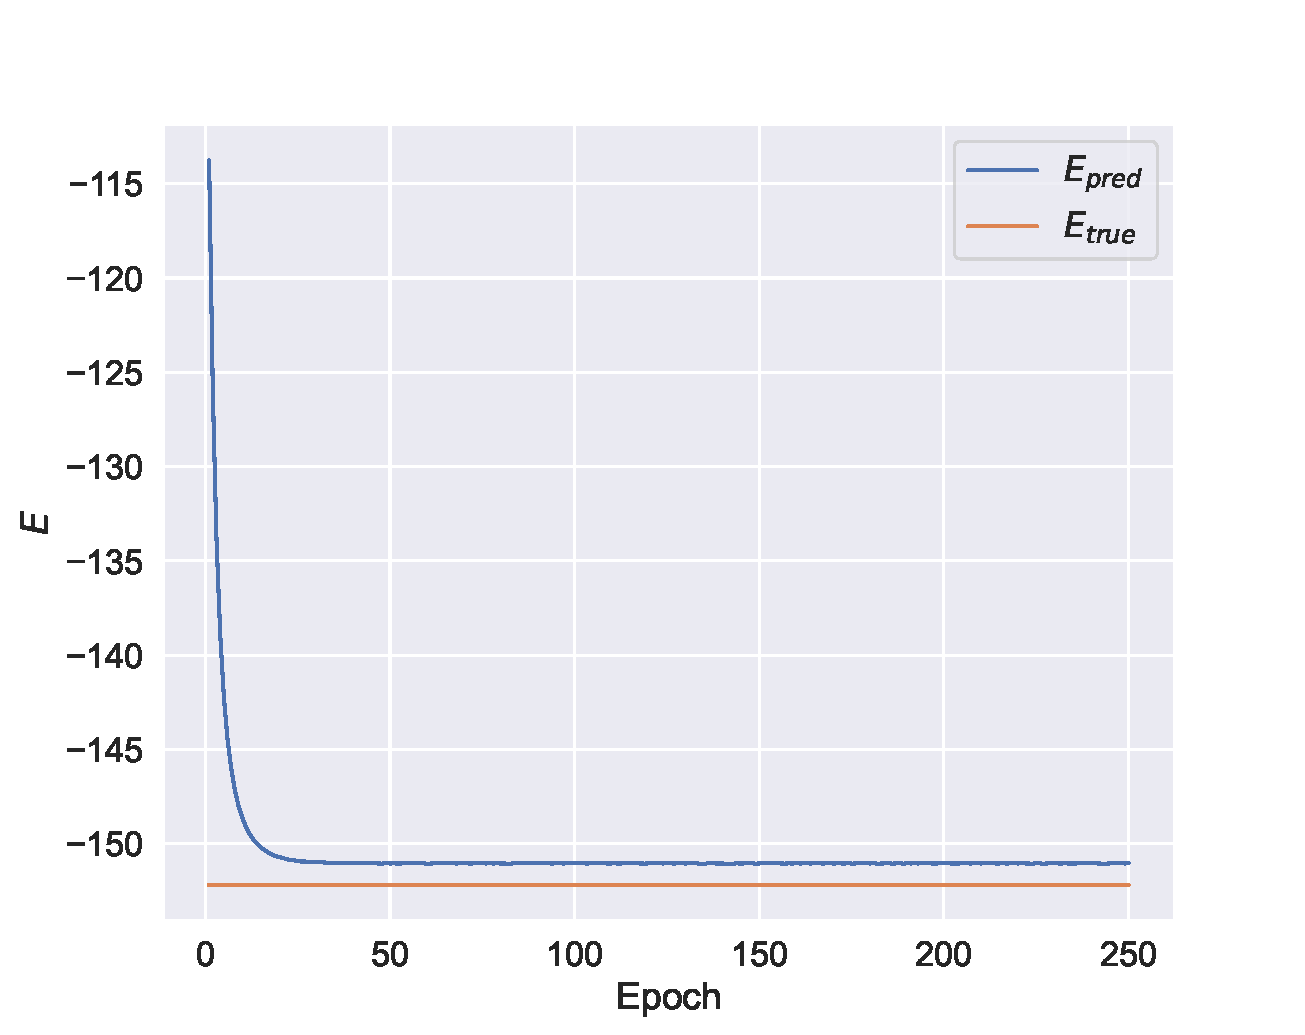
\includegraphics[width=0.95\textwidth]{Figures/Plots/Lipkin/Result25conv.pdf}
  \end{center}
  \caption{The convergence of the predicted ground state energy for the Lipkin model with $25$ particles, $\varepsilon = 2$, $V = -1$ and $W=0$.}\label{fig:res25conv}
\end{figure}

Where the final predicted energy is $E_{rbm} = -151.0 \pm 8.8$. The RBM converge towards a value that is slightly above the true value, and this is seemingly the closest the RBM manages to get. If we look at the gradients for the visual and hidden bias we see that they approach zero:

\begin{figure}[H]
  \begin{center}
    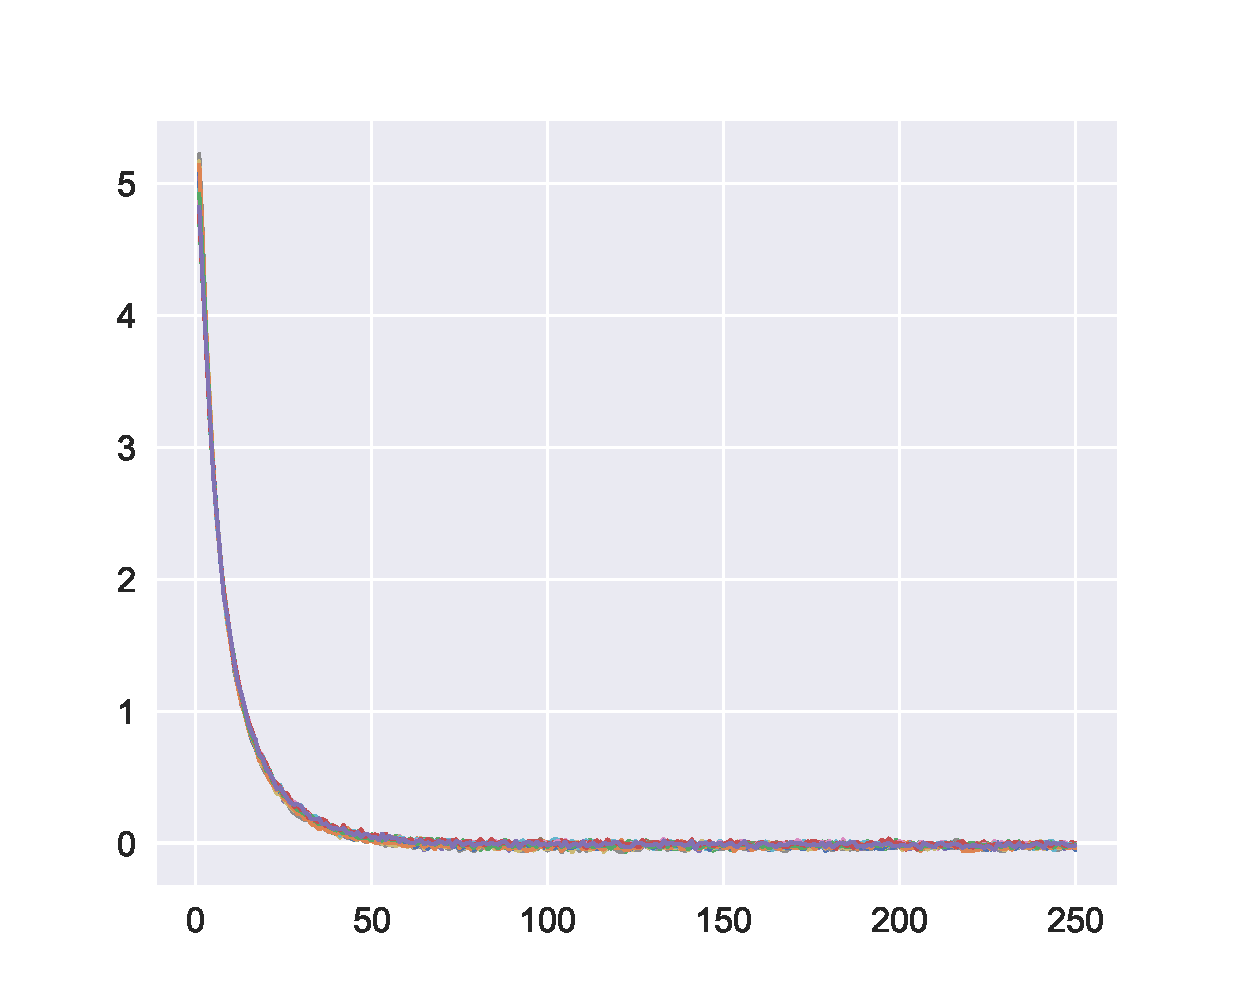
\includegraphics[width=0.95\textwidth]{Figures/Plots/Lipkin/Result25dvb}
  \end{center}
  \caption{The convergence of the gradient with respect to the visual layer bias. Lipkin model with $25$ particles, $\varepsilon = 2$, $V = -1$ and $W=0$.}
\end{figure}

\begin{figure}[H]
  \begin{center}
    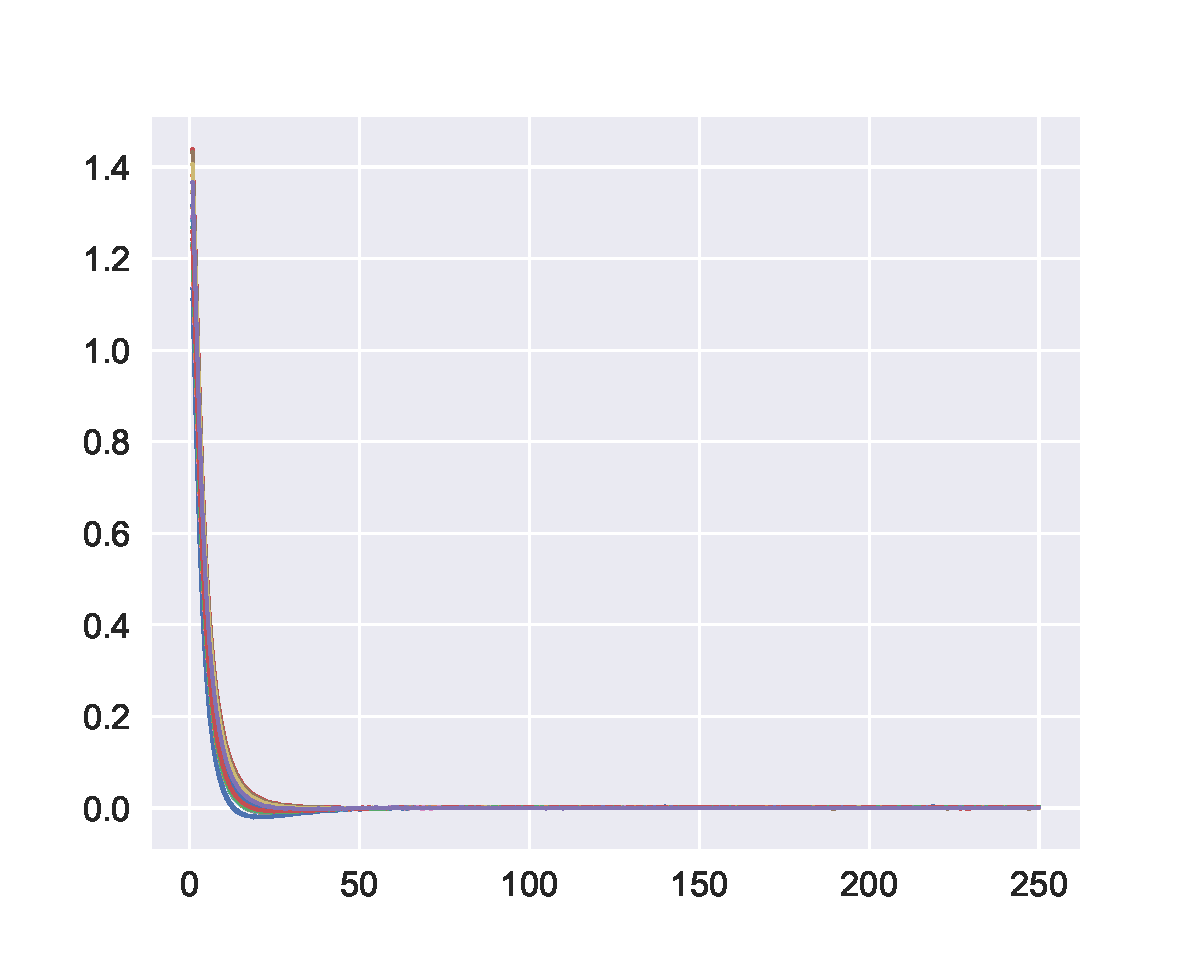
\includegraphics[width=0.95\textwidth]{Figures/Plots/Lipkin/Result25dhb}
  \end{center}
  \caption{The convergence of the gradient with respect to the hidden layer bias. Lipkin model with $25$ particles, $\varepsilon = 2$, $V = -1$ and $W=0$. As there are twenty five of the dimensionless variables we have refrained from adding a legend.}
\end{figure}

Where we see that both has converged to zero, which means that the RBM has found its solution with the most even local energy between its samples, but it is important to remember that the $\Psi_{rbm}$ is not the exact wavefunction, and since we have

$$E_{rbm} \geq E_0 \; ,$$

the machines best approximation of it is always a higher energy, as seen in \ref{fig:res25conv}.

\subsection{The effect of \texorpdfstring{$\varepsilon$}{epsilon} on RBM prediction accuracy}
First we see how the RBM performs for $\varepsilon$ values with only pair excitation $V=-1$ and $W=0$.

\begin{figure}[H]
  \begin{center}
    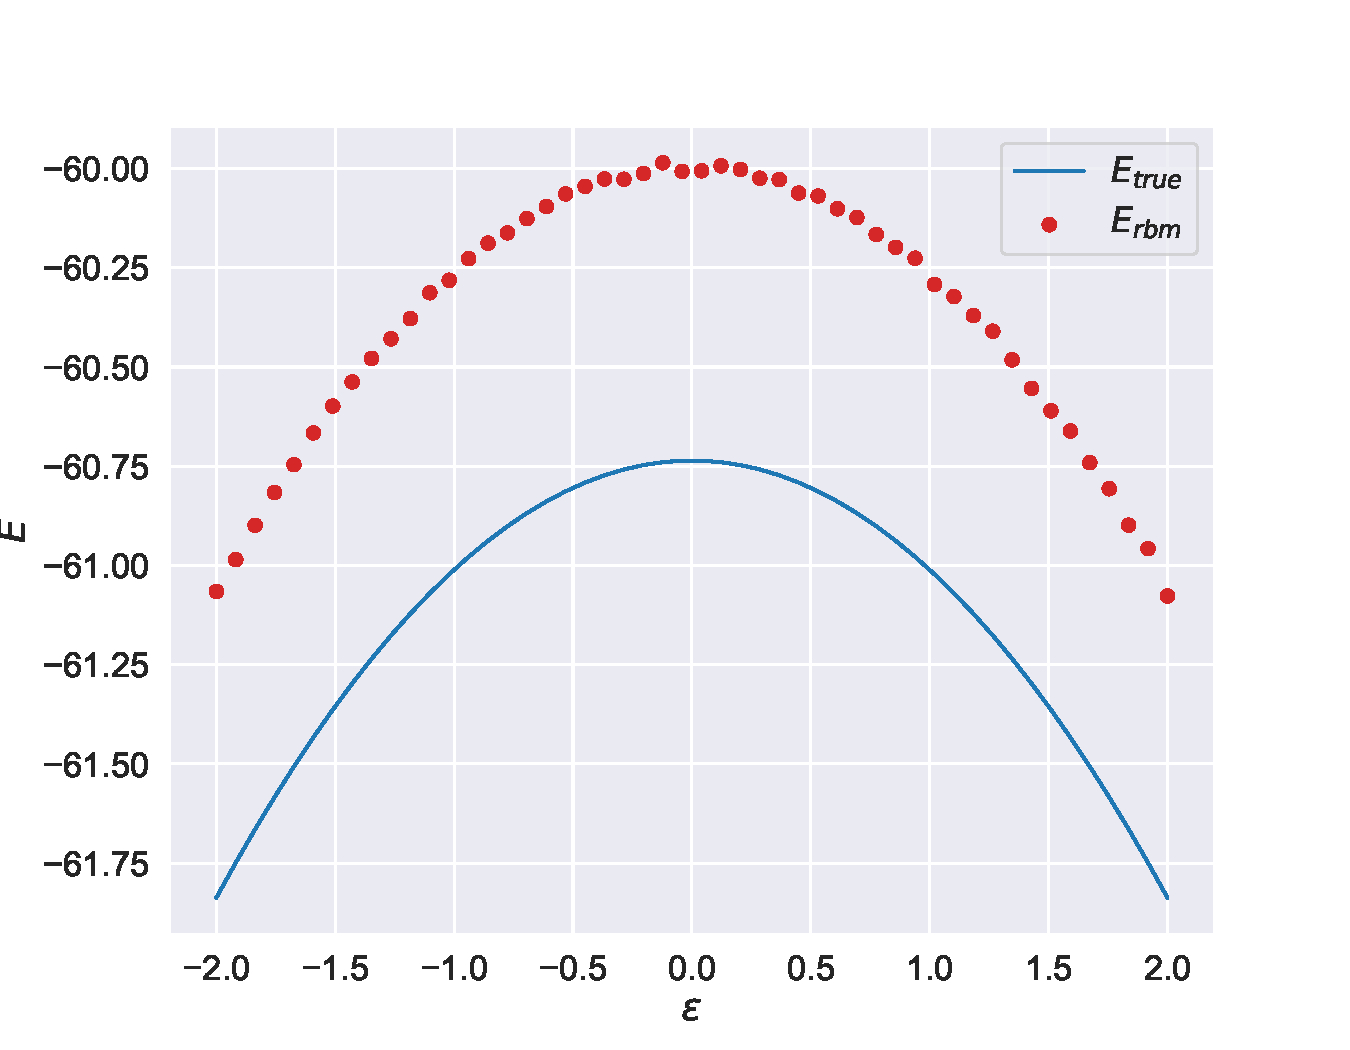
\includegraphics[width=0.95\textwidth]{Figures/Plots/Lipkin/val-true[eps][-2.0-2.0][e=500][n=16][V=-1][W=0].pdf}
  \end{center}
  \caption{The RBM prediction of the ground state energy for the Lipkin system with $V=-1$ and $W=0$ and $16$ particles.}
\end{figure}

The gap between the RBM prediction and the true value seen in \ref{fig:res25conv} is seen here as well, as the RBM misses by quite a bit for the whole range. Interestingly the error seems to be somewhat consistent around $0.75$ for all the $\varepsilon$ values. Further we take a look at the impact that $\varepsilon$ has on the RBM accuracy when we include interaction strength as well. We set $W=0.5$ and get:

\begin{figure}[H]
  \begin{center}
    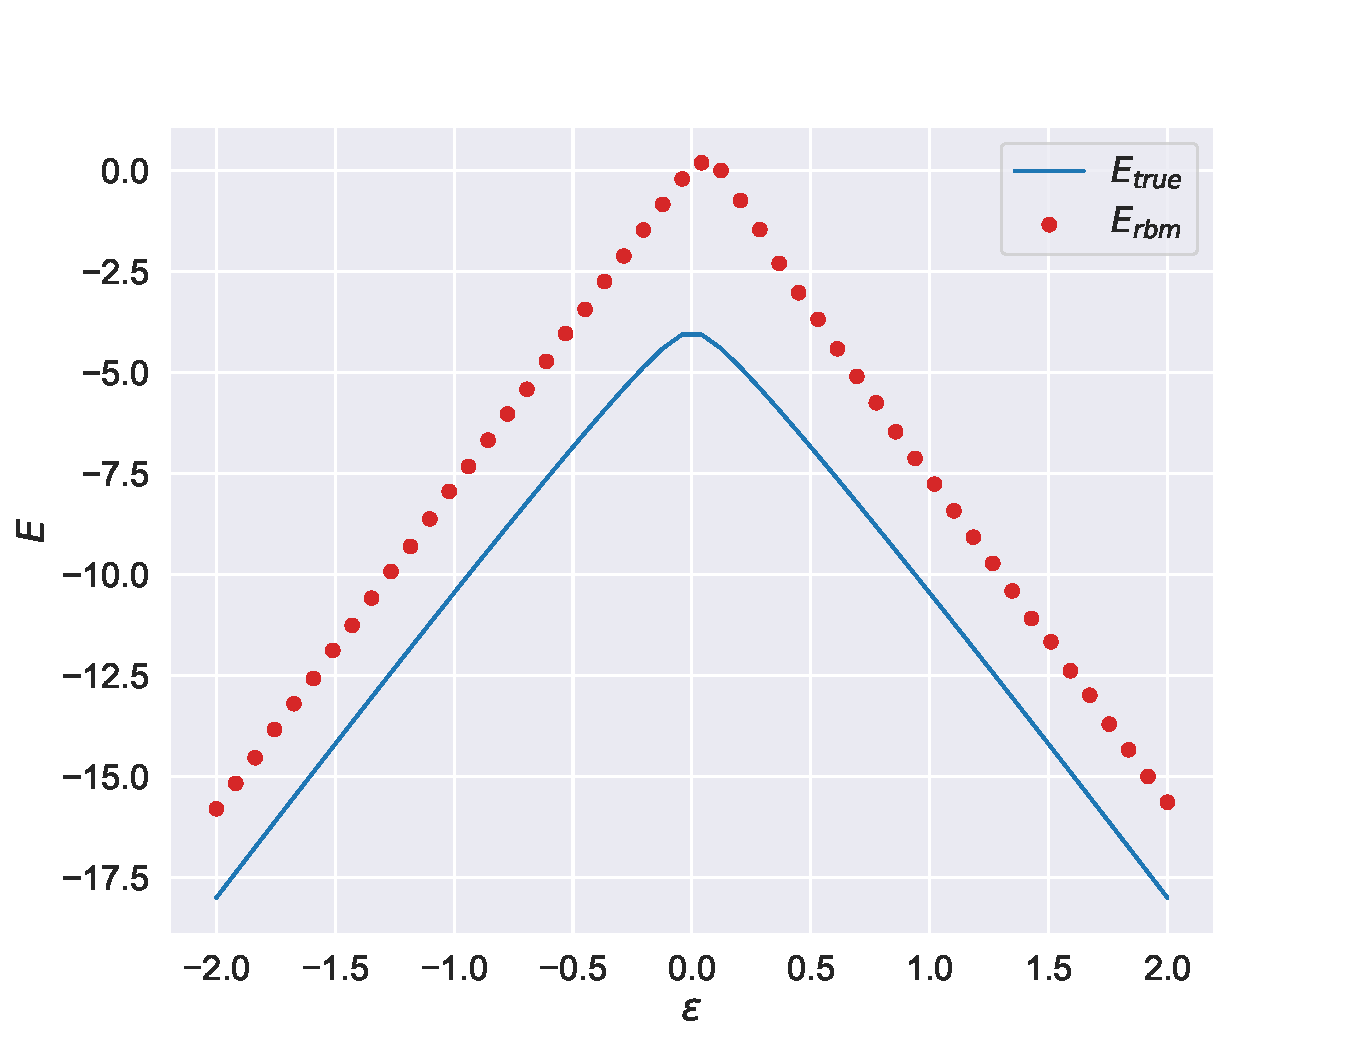
\includegraphics[width=0.95\textwidth]{Figures/Plots/Lipkin/val-true[eps][-2.0-2.0][e=850][n=16][V=-0.5][W=0.5].pdf}
  \end{center}
  \caption{The RBM prediction of the ground state energy for the Lipkin system with $V=-1$ and $W=0.5$ and $16$ particles.}
\end{figure}

Here we still see the RBM prediction being quite a bit higher than the true ground state energy, though now the error increases sharply towards $\varepsilon = 0$.

\subsection{The effect of \texorpdfstring{$V$}{V} on RBM prediction accuracy}

Looking at the pair excitation strength we set $\varepsilon = -2$ instead, and we get:

\begin{figure}[H]
  \begin{center}
    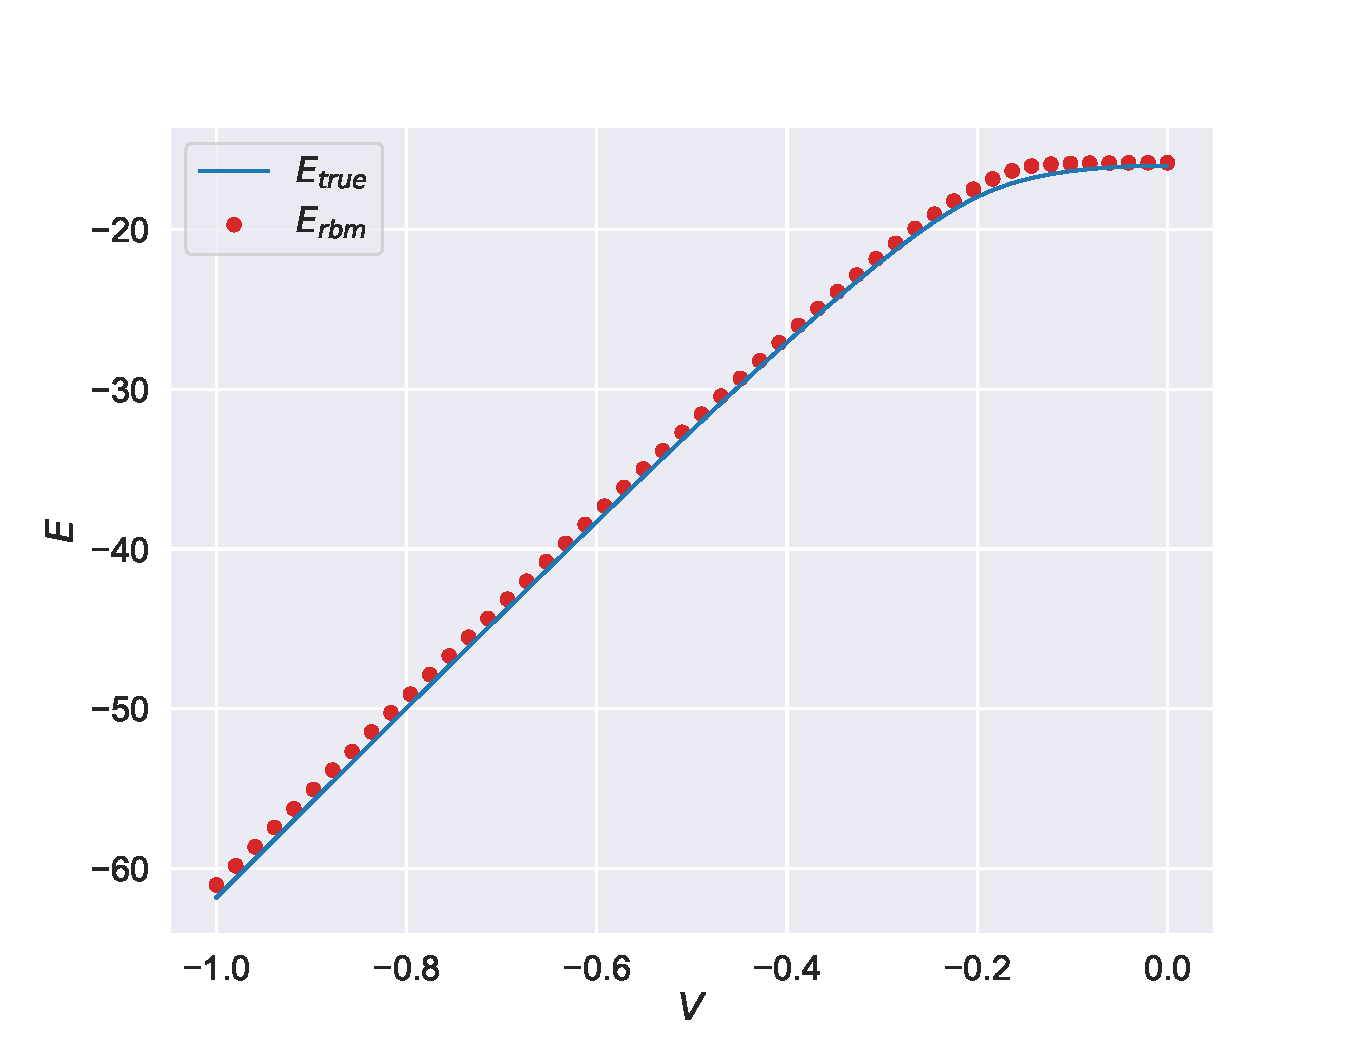
\includegraphics[width=0.95\textwidth]{Figures/Plots/Lipkin/val-true[V][-1.0-0.0][e=850][n=16][eps=-2][W=0].pdf}
  \end{center}
  \caption{The RBM prediction of the ground state energy for the Lipkin system with $\varepsilon=-2$ and $W=0$ and $16$ particles.}
\end{figure}

It is important to note that the scale of the y-axis has increased, so we the gap between the RBM prediction and the true value is harder to distinguish. Still we see the gap decrease slightly from $V=-1$ towards $V=-0.2$ where the RBM prediction defaults to the $V=0$ case. If we introduce the spin exchange interaction as well with $W=0.1$ we get:

\begin{figure}[H]
  \begin{center}
    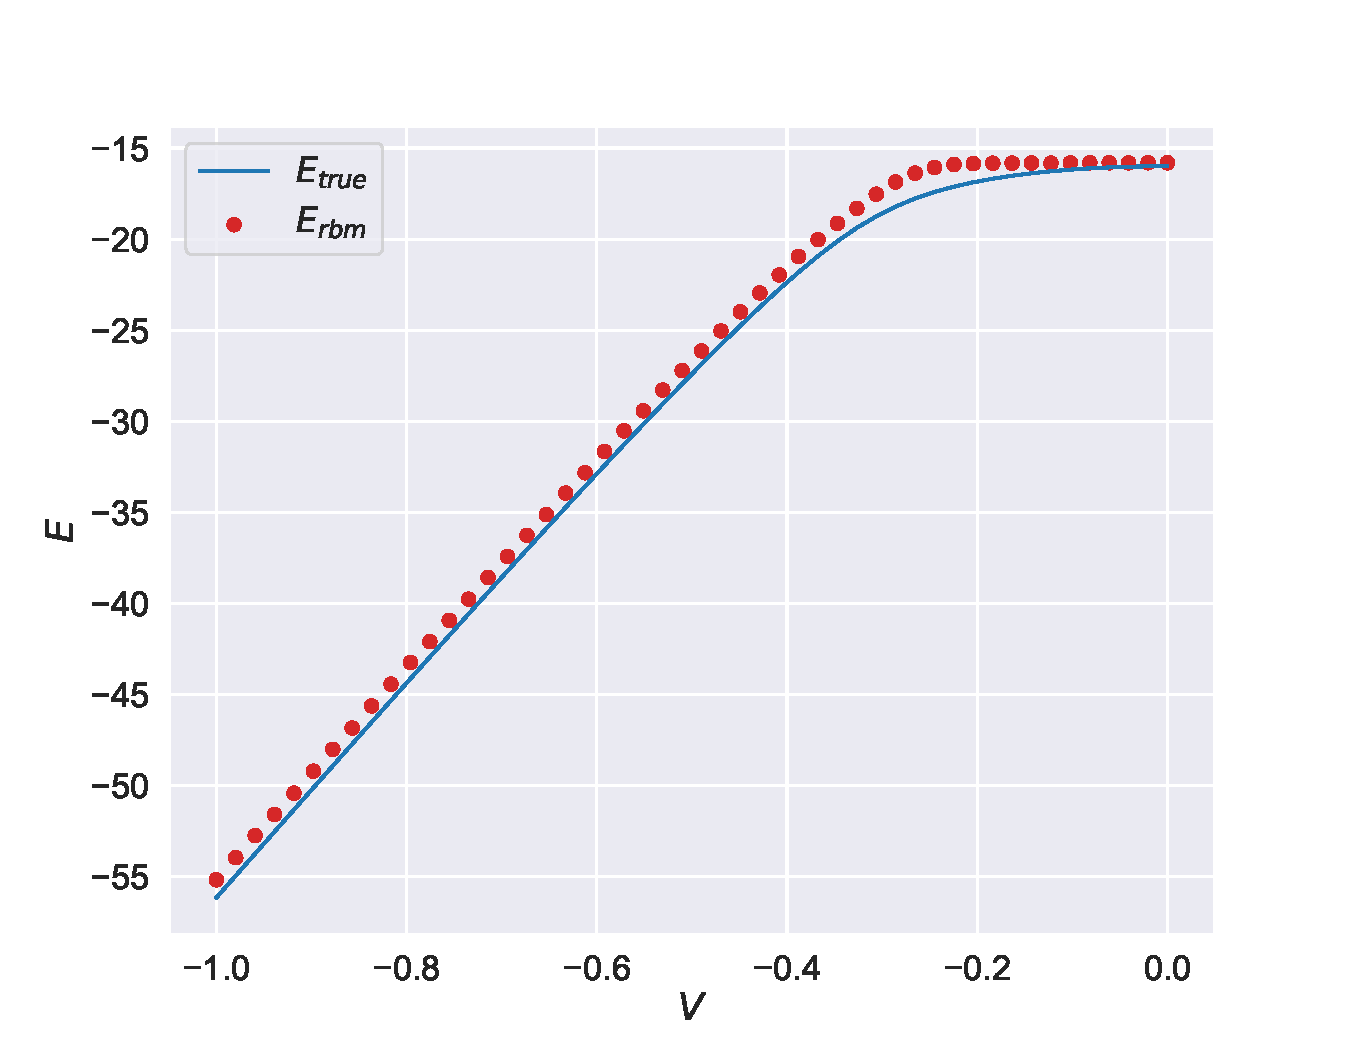
\includegraphics[width=0.95\textwidth]{Figures/Plots/Lipkin/val-true[V][-1.0-0.0][e=850][n=16][eps=-2][W=0.1].pdf}
  \end{center}
  \caption{The RBM prediction of the ground state energy for the Lipkin system with $\varepsilon=-2$ and $W=0.1$ and $16$ particles.}
\end{figure}

And here the behaviour towards $V=0$ is even more accentuated.

\subsection{The effect of \texorpdfstring{$W$}{W} on RBM prediction accuracy}

We check the $W$ spin exchange interaction strength first with $V=0$, and we get:

\begin{figure}[H]
  \begin{center}
    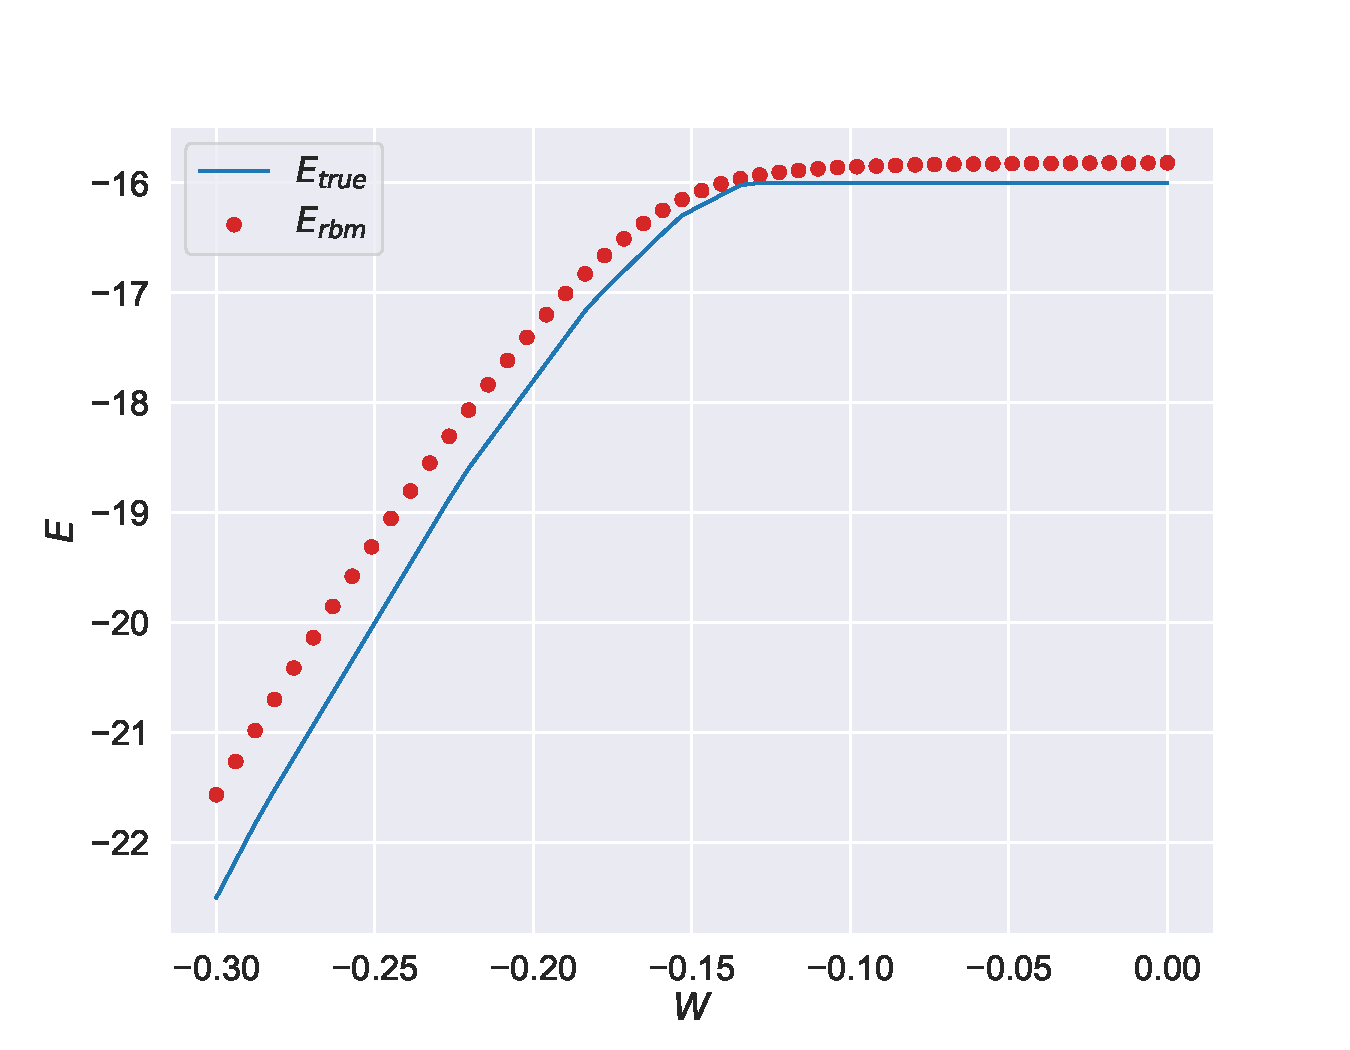
\includegraphics[width=0.95\textwidth]{Figures/Plots/Lipkin/val-true[W][-0.3-0.0][e=850][n=16][eps=-2][V=0].pdf}
  \end{center}
  \caption{The RBM prediction of the ground state energy for the Lipkin system with $\varepsilon=-2$ and $V=0$ and $16$ particles.}
\end{figure}

Where we see a clear decrease in the error at $W=-0.15$. At lower values of $W$ the RBM prediction error only seems to increase, though this may be of the increasing absolute value of the ground state energy. Together with pair excitation we get that the accuracy evolves as follows:

\begin{figure}[H]
  \begin{center}
    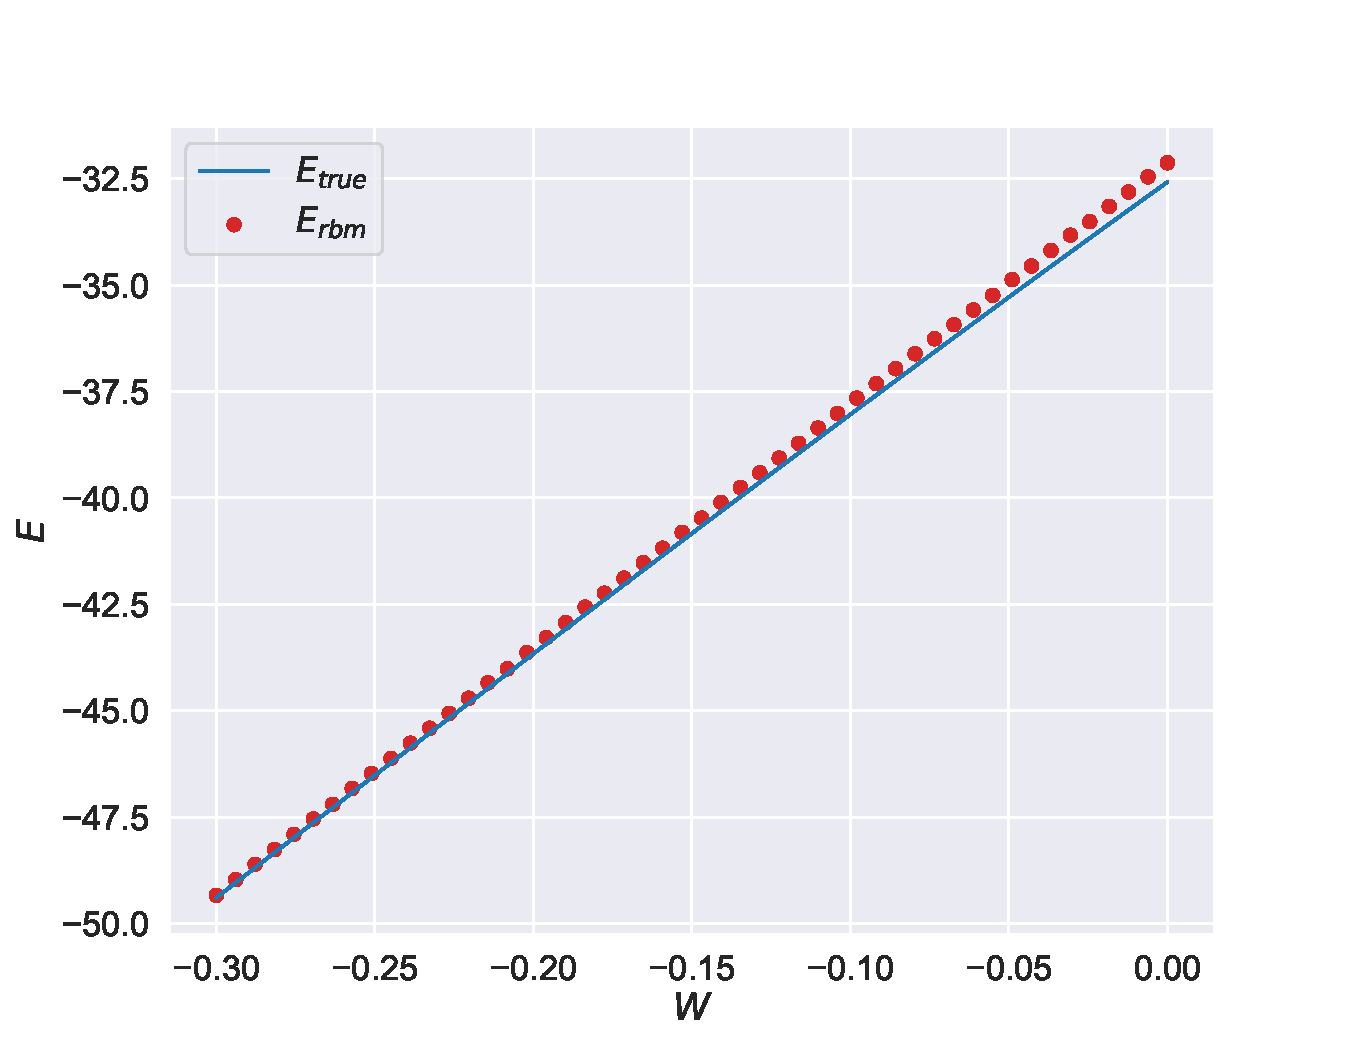
\includegraphics[width=0.95\textwidth]{Figures/Plots/Lipkin/val-true[W][-0.3-0.0][e=850][n=16][eps=-2][V=-0.5].pdf}
  \end{center}
  \caption{The RBM prediction of the ground state energy for the Lipkin system with $\varepsilon=-2$ and $V=-0.5$ and $16$ particles.}
\end{figure}

With the pair excitation the RBM prediction seem to favour lower $W$ values instead.

\subsection{System size effect on the RBM}

We plot the variance at the different system sizes for the Lipkin model with $\varepsilon =-2$, $V=-0.5$ and $W=0.1$.

\begin{figure}[H]
  \begin{center}
    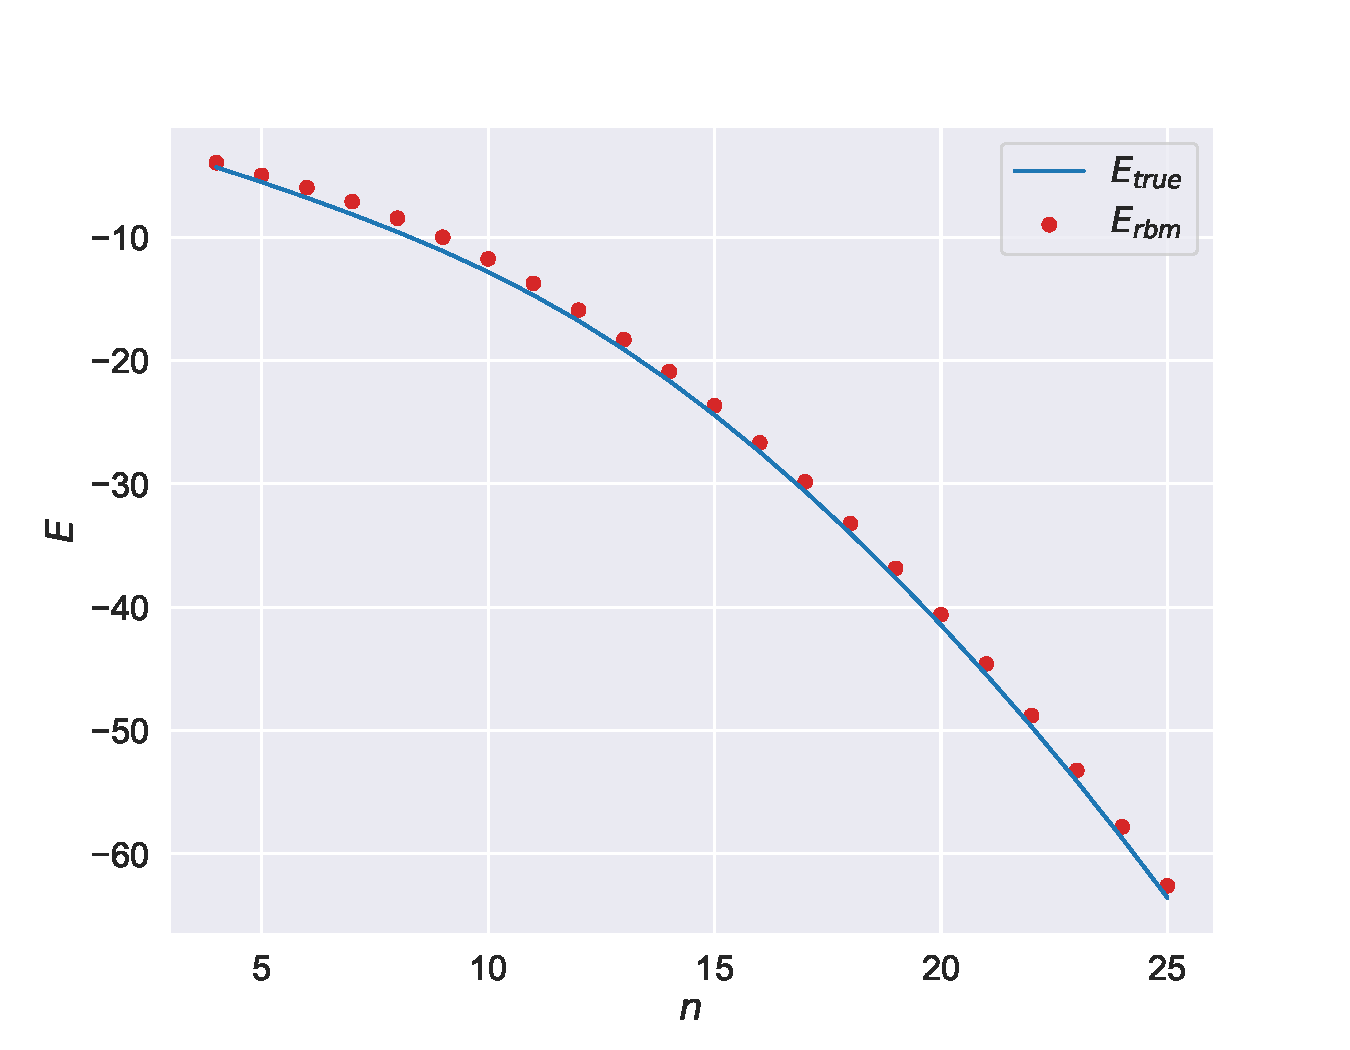
\includegraphics[width=0.95\textwidth]{Figures/Plots/Lipkin/val-true[particles][4-25][e=850][eps=-2][V=-0.5][W=0.1].pdf}
  \end{center}
  \caption{The RBM prediction of the ground state energy for the Lipkin system with $\varepsilon=-2$ and $V=-0.5$ and $W=0.1$.}
\end{figure}

The error stays almost the same throughout the different system sizes, but this means the relative error must go down, as we can see here:

\begin{figure}[H]
  \begin{center}
    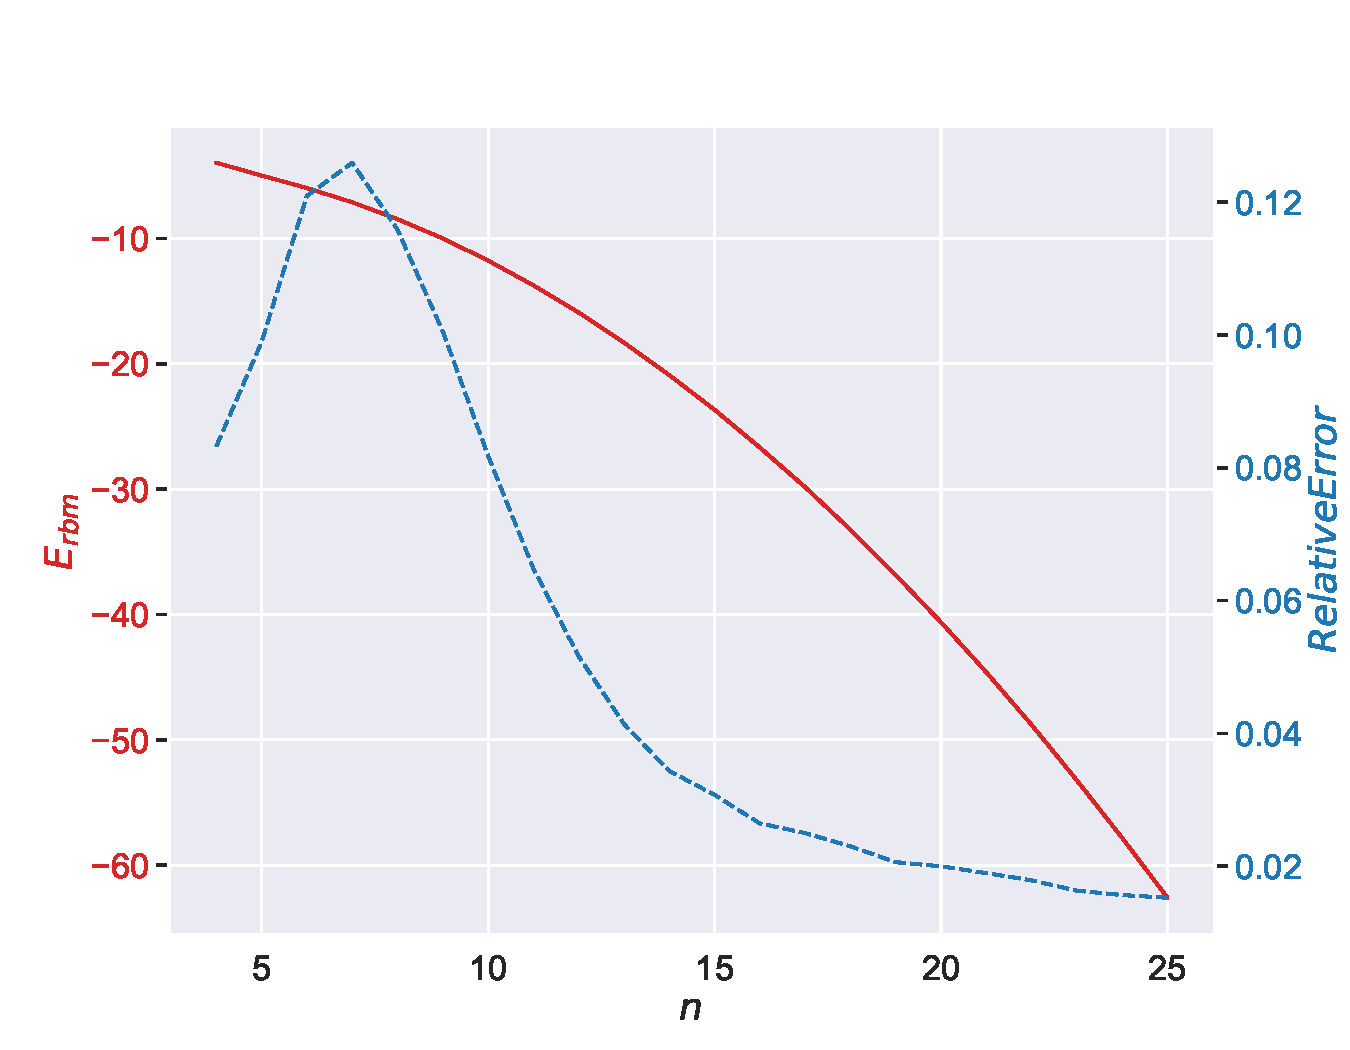
\includegraphics[width=0.95\textwidth]{Figures/Plots/Lipkin/[particles][4-25][e=850][eps=-2][V=-0.5][W=0.1]error.pdf}
  \end{center}
  \caption{The RBM prediction of the ground state energy for the Lipkin system with $\varepsilon=-2$ and $V=-0.5$ and $W=0.1$ and the relative error for different quantum system sizes.}
\end{figure}




